\documentclass[twoside]{article}

\usepackage[sc]{mathpazo}
\usepackage[utf8]{inputenc}
\usepackage[english,italian]{babel}
\linespread{1.05} % Line spacing - Palatino needs more space between lines
\usepackage{microtype} % Slightly tweak font spacing for aesthetics

\usepackage{graphicx}
\usepackage[hmarginratio=1:1,top=32mm,columnsep=20pt]{geometry} % Document margins
\usepackage{multicol} % Used for the two-column layout of the document
\usepackage[hang, small,labelfont=bf,up,textfont=it,up]{caption} % Custom captions under/above floats in tables or figures
\usepackage{booktabs} % Horizontal rules in tables
\usepackage{float} % Required for tables and figures in the multi-column environment - they need to be placed in specific locations with the [H] (e.g. \begin{table}[H])
\usepackage{hyperref} % For hyperlinks in the PDF

\usepackage{lettrine} % The lettrine is the first enlarged letter at the beginning of the text
\usepackage{paralist} % Used for the compactitem environment which makes bullet points with less space between them

\usepackage{abstract} % Allows abstract customization
\renewcommand{\abstractnamefont}{\normalfont\bfseries} % Set the "Abstract" text to bold
\renewcommand{\abstracttextfont}{\normalfont\small\itshape} % Set the abstract itself to small italic text

\usepackage{titlesec} % Allows customization of titles
\renewcommand\thesection{\Roman{section}} % Roman numerals for the sections
\renewcommand\thesubsection{\Roman{subsection}} % Roman numerals for subsections
\titleformat{\section}[block]{\large\scshape\centering}{\thesection.}{1em}{} % Change the look of the section titles
\titleformat{\subsection}[block]{\large}{\thesubsection.}{1em}{} % Change the look of the section titles

%\usepackage{fancyhdr} % Headers and footers
%\pagestyle{fancy} % All pages have headers and footers
%\fancyhead{} % Blank out the default header
%\fancyfoot{} % Blank out the default footer
%\fancyhead[C]{$\bullet$ Gennaio 2016 $\bullet$} % Custom header text
%\fancyfoot[RO,LE]{\thepage} % Custom footer text

\usepackage{amsmath}

\usepackage{biblatex}
\bibliography{bibliography}

\setlength\parindent{0pt} % Nessuna rientranza ad inizio paragrafo
\setlength\parskip{10pt} % Spaziatura tra paragrafi

%----------------------------------------------------------------------------------------
% IMPOSTAZIONI DI FANCYHDR
%----------------------------------------------------------------------------------------

\hyphenation{dynamo baseball}

%----------------------------------------------------------------------------------------
%	CUSTOM MACRO
%----------------------------------------------------------------------------------------

\newcommand{\vclock}{\mathrm{VC}} % VC

%----------------------------------------------------------------------------------------
%	TITLE SECTION
%----------------------------------------------------------------------------------------

\title{\vspace{-15mm}\fontsize{24pt}{10pt}\selectfont\textbf{Consistency and Replication}} % Article title

\author{
\large
\textsc{Bartolomeo Lombardi, Amerigo Mancino, Andrea Segalini}\\[2mm] % Your name
\normalsize Università degli Studi di Bologna % Your institution
\vspace{5mm} \\
\normalsize \href{mailto:bartolomeo.lombardi@studio.unibo.it}{bartolomeo.lombardi@studio.unibo.it}\\
\normalsize \href{mailto:amerigo.mancino@studio.unibo.it}{amerigo.mancino@studio.unibo.it}\\
\normalsize \href{mailto:andrea.segalini@studio.unibo.it}{andrea.segalini@studio.unibo.it}
\vspace{-5mm}
}
\date{Gennaio 2016}

%----------------------------------------------------------------------------------------

\begin{document}
\maketitle 
%\thispagestyle{fancy} % All pages have headers and footers

%----------------------------------------------------------------------------------------
%	ABSTRACT
%----------------------------------------------------------------------------------------

\begin{abstract}
\noindent
Sistemi di storage moderni replicano i dati su più macchine al fine di garantirne persistenza, low latency e tolleranza ai guasti. La presenza di più repliche di un medesimo dato genera quindi problemi di coerenza fra i dati stessi. Tale coerenza può essere garantita mediante diversi modelli, ognuno con i propri punti di forza e le proprie debolezze. Chiaramente, non ne esiste uno valido in generale e la scelta deve essere fatta tenendo in considerazione quali proprietà del sistema riteniamo maggiormente rilevanti ai nostri scopi. Pertanto, prendendo in esame i due sistemi di key-value store distribuiti Amazon Dynamo e COPS, è stato possibile verificare, anche tramite confronti, come questi compromessi vengono raggiunti.
\end{abstract}

%----------------------------------------------------------------------------------------

\vspace{20mm} % Spaziatura tra abstract e corpo articolo

%----------------------------------------------------------------------------------------
%	ARTICLE CONTENTS
%----------------------------------------------------------------------------------------

\begin{multicols}{2} % Two-column layout throughout the main article text

\section{Introduzione}
\label{sec:introduzione}
\lettrine[nindent=0em,lines=2]{O} gni applicazione necessita di un livello di coerenza che cambia a seconda degli scopi che vuole raggiungere e delle priorità che vuole ottenere. Infatti, nel 2000 è stato congetturato, e successivamente dimostrato, un risultato teorico che prova che in ogni sistema distribuito non è possibile soddisfare contemporaneamente tutte e tre le seguenti proprietà: \emph{availability}, ossia ogni richiesta riceve sempre una risposta su ciò che è riuscito o fallito non rimanendo mai in attesa indefinitamente, \emph{partition-tolerance}, ossia il sistema continua a funzionare nonostante arbitrarie perdite di messaggi, \emph{consistency}, ossia tutti i nodi vedono gli stessi dati simultaneamente. Questa conclusione è stata dimostrata nel 2002, dopo quasi trenta anni di ricerca, e va sotto il nome di Teorema CAP.
Per descrivere alcuni differenti modelli di coerenza, utilizzeremo come esempio i punteggi di una partita di baseball, memorizzati all'interno di un key-value store distribuito, come mostrato di seguito:
\begin{table}[H]
\centering
\resizebox{\columnwidth}{!}{%
\begin{tabular}{l*{10}{c}r}
\textbf{Team} & \textbf{1} & \textbf{2} & \textbf{3} & \textbf{4} & \textbf{5} & \textbf{6} & \textbf{7} & \textbf{8} & \textbf{9} & \textbf{RUNS} \\
\hline
\textbf{Visitors}     & 0 & 0 & 1 & 0 & 1 & 0 & 0 &  &  & 2 \\
\textbf{Home}         & 1 & 0 & 1 & 1 & 0 & 2 &   &  &  & 5 \\
\end{tabular}
}
\caption{Esempio di punteggio nel baseball.}
\label{tab:punteggio-baseball}
\end{table}

\textbf{Strong consistency.} La garanzia più alta che possiamo raggiungere fornisce ad ogni client che effettua operazioni di lettura sempre l'ultimo valore aggiornato. Per implementare tale livello, è necessario un alto livello di sincronizzazione tra i vari nodi, che per essere raggiunto esige attese, causando un calo delle performance e la partecipazione attiva di tutti i nodi. In riferimento all'esempio, è possibile che ci venga ritornato unicamente il punteggio 2-5.

\textbf{Eventual Consistency.} Formalmente l'eventual consistency consente di ritornare un qualunque valore che è stato scritto su un dato che il client vuole leggere. In pratica, quello che questo livello garantisce è che se non vengono eseguiti nuovi aggiornamenti su un oggetto, eventualmente tutti gli accessi a quell'oggetto ritorneranno l'ultimo valore aggiornato.

\section{Dettagli Tecnici}
\label{sec:dettagli-tecnici}
%\lettrine[nindent=0em,lines=2]{I}
In questa sezione prendiamo in considerazione due noti sistemi di storage distribuiti: \emph{COPS} (\emph{Cluster of Order Preserving Service}) e \emph{Amazon Dynamo}. Il primo è un sistema distribuito su scala geografica (quella che viene definita in gergo come “wide area”) con repliche identiche degli stessi dati dislocate in più datacenter. Il secondo, invece, è costituito da nodi, potenzialmente disposti in più datacenter distinti, in cui sono distribuiti e replicati i dati. La specifica afferma che in COPS questi dati non sono partizionati fra i vari datacenter che formano il sistema, ma replicati tra essi, mentre in Dynamo sono divisi nei diversi nodi e di ogni elemento ne esistono più copie.

\textbf{Replicazione.} Per affrontare il problema della replicazione dobbiamo innanzi tutto sottolineare come in COPS ogni datacenter possieda una replica di tutti i dati, mentre in Dynamo la questione diventa più complessa, in quanto i dati non sono replicati su tutti i nodi ma solo su un numero $N$ (dove $N$ è un intero molto minore del numero totale di nodi di cui il sistema dispone). Inoltre, in quest'ultimo il partizionamento dei dati viene gestito tramite la tecnica del \emph{Consistent Hashing} \cite{jade:book}, che considera una tabella hash chiusa ad anello e con nodi disposti su di esso, al fine di delimitare gli intervalli con cui sono partizionati i dati (figura \ref{fig:consistent-hashing-ring}).
\begin{figure}[H]
\centering
\resizebox{\columnwidth}{!}{%
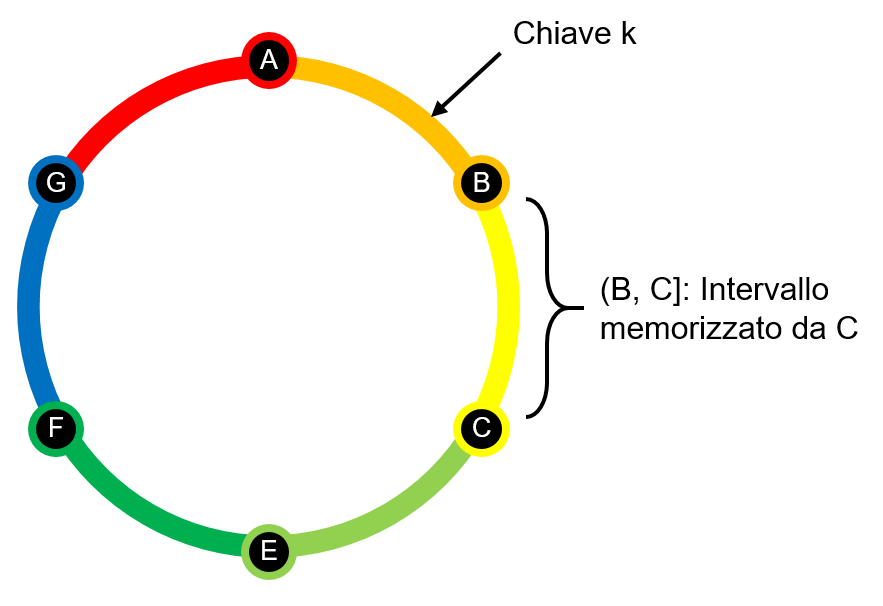
\includegraphics{img/consistent-hashing-ring.png}
}
\caption{Schematizzazione del Consistent Hashing}
\label{fig:consistent-hashing-ring}
\end{figure}

\textbf{Versionamento.} La presenza di repliche necessita l'aggiunta di informazioni ausiliarie per tracciare le versione e poter risolvere eventuali conflitti. In COPS ad ogni aggiornamento viene associato un \emph{Lamport timestamp} [ref], costituito da un clock logico e dall'identificativo univoco del nodo, che è tale da fornire un ordinamento globale. Mediante questo espediente, è possibile implementare una \emph{last-writer-win-rule}, garantendo, in caso di conflitti, la vittoria della scrittura con timestamp maggiore. In Dynamo invece la tecnica adottata è quella dei \emph{Vector clock} [ref] che introduce un vettore di coppie $<\mathrm{id\char`_nodo}, \mathrm{counter}>$, abbinato ad ogni dato replicato. Ogni volta che un nodo compie una modifica, incrementa il proprio counter; date quindi due versioni $x$ e $y$ del medesimo oggetto e denotato con $\vclock(x)_z$ il vector clock relativo al nodo $z$, abbiamo che vale:
\begin{multline*}
\vclock(x) < \vclock(y) \iff \\
\big( \forall z \mathrel{:} \vclock(x)_z \leq \vclock(y)_z \big) \\
\land \big( \exists z' \mathrel{:} \vclock(x)_{z'} < \vclock(y)_{z'} \big)
\end{multline*}
Chiaramente, l’approccio intrapreso da Dynamo consente di tracciare branch di versioni parallele ed operare una riconciliazione definita dal client, mentre in COPS, data la natura totale dell'ordinamento, in caso di conflitto, verrebbe sicuramente perso uno dei due rami divergenti. In quest'ultimo caso, la scelta fatta garantisce quindi una notevole semplicità nell'applicazione, mentre, al contrario, in Dynamo è necessario prevedere e gestire la ricezione di versioni concorrenti. Inoltre, la dimensione del vector clock può crescere molto, soprattutto in presenza di numerosi fallimenti, rendendo onerose le operazioni di analisi su di essi.

\textbf{Coerenza.} In COPS implementiamo \emph{causal+ consistency}, in quanto si vuole garantire la coerenza più forte possibile che permetta, al contempo, di soddisfare le caratteristiche \emph{ALPS} [ref?], nel rispetto del Teorema CAP. È impossibile quindi implementare livelli di coerenza maggiori, quali la strong consistency o la sequential consistency. In dettaglio, la causal+ consistency viene definita come la combinazione di due componenti: la causal consistency, definita nella Sezione \ref{sec:introduzione}, e la \emph{convergent conflict handling}, che garantisce che tutte le operazioni di \texttt{put} in conflitto vengano gestite allo stesso modo da tutti i nodi usando una funzione $h$ associativa e commutativa.
In Dynamo, sono implementati due modelli di coerenza, strong consistency ed eventual consistency, impostabili mediante dei parametri che governano direttamente anche performance, availability e persistenza dei dati. Questi ultimi parametri, sempre nel rispetto del Teorema CAP, consentono di bilanciare il sistema, permettendone un diverso uso in base alle esigenze.

\textbf{Coerenza in Dynamo}. La coerenza delle operazioni è gestita con la tecnica del \emph{Quorum} [cite]. Il sistema permette di impostare due parametri: il numero di nodi dai quali viene atteso un acknowledge a seguito di una scrittura, detto $W$, e il numero di nodi che partecipa ad un'operazione di lettura, detto $R$. Facendo riferimento alla Figura \ref{fig:get}, nell'operazione di lettura, il client contatta il nodo A che diventa il coordinatore della richiesta e poi i restanti $N-1$ nodi che mantengono la replica del dato. Dopo aver cercato nella propria memoria secondaria il valore, A aspetta la risposta da almeno $R-1$ nodi (non $R$, poiché A stesso è conteggiato). I valori ritornati, a questo punto, possono appartenere tutti alla medesima versione, quindi essere tutti coerenti, oppure presentare versioni precedenti/successive o concorrenti. L'ordinamento parziale dalle versioni è ottenuto analizzando i vector clock degli oggetti. In caso di ordinamento esistente, il conflitto è risolto da A prendendo l'ultima versione, viceversa sono tornate al client tutte le versioni concorrenti collezionate, lasciando a quest'ultimo il compito di riunificare la biforcazione. L'operazione di scrittura (Figura \ref{fig:put}) avviene in maniera analoga: a differenza dei valori vengono aspettati gli acknowledge di conferma sulla scrittura avvenuta.
\begin{figure}[H]
\centering
\resizebox{\columnwidth}{!}{%
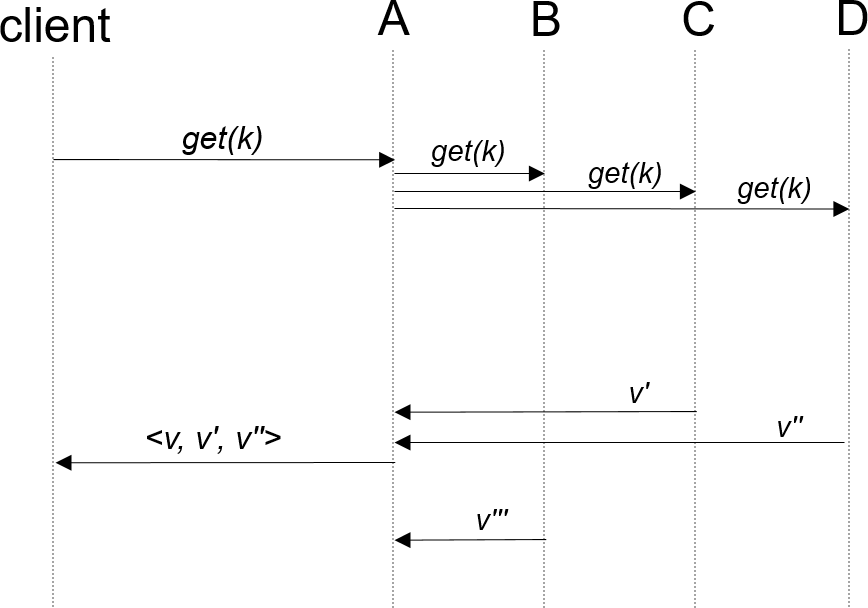
\includegraphics{img/get.png}
}
\caption{Timeline dell'esecuzione di \texttt{get(k)}}
\label{fig:get}
\end{figure}
\begin{figure}[H]
\centering
\resizebox{\columnwidth}{!}{%
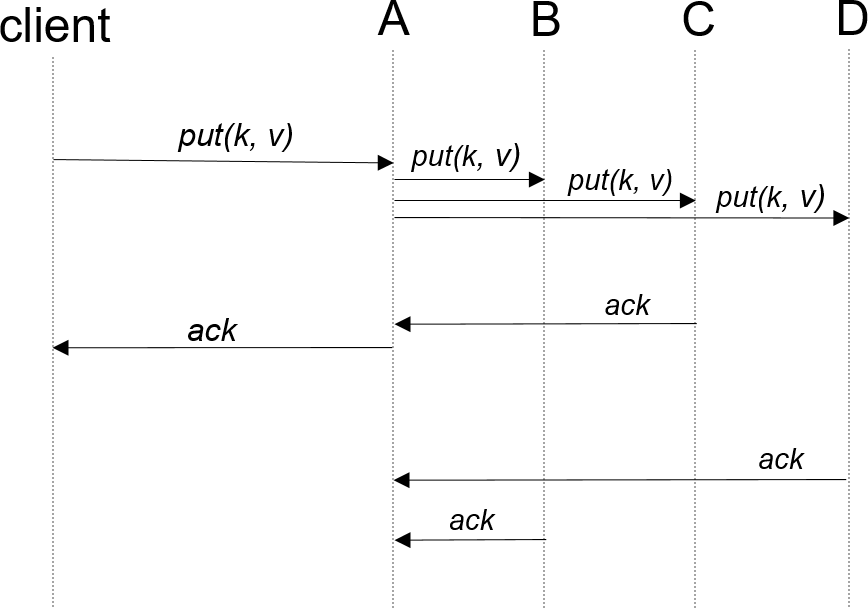
\includegraphics{img/put.png}
}
\caption{Timeline dell'esecuzione di \texttt{put(k, v)}}
\label{fig:put}
\end{figure}
I parametri $W$ e $R$ mediano tra coerenza, availability, performance e persistenza dei dati. Se $W+R > N$ allora l'insieme dei nodi che hanno effettuato sicuramente l'ultima scrittura nel sistema si interseca con l'insieme dei nodi che rispondono in caso di lettura. Dunque abbiamo garanzia che l'ultimo valore scritto per una certa chiave sia ritornato sicuramente in caso di lettura poiché esiste almeno un nodo che lo possiede e che risponde alla richiesta. La garanzia di ritorno dell'ultima versione scritta corrisponde ad una strong consistency. Come ripetuto diverse volte, avere tale modello di coerenza implica la perdita di altre qualità. Alti valori di $W$ e $R$ comportano performance peggiori poiché sono attese un maggior numero di risposte ad ogni richiesta, allo stesso modo peggiora l'availability poiché sono necessari un maggior numero di nodi per completare un'operazione. In generale il sistema è usato in configurazione $W+R \leq N$ che implica il modello eventual consistency. Tuttavia più il valore $W+R$ si avvicina ad $N$, più aumenta la probabilità che i due insiemi sopracitati si intersechino e quindi l'ultimo valore letto sia anche l'ultimo scritto.

\section{Conclusioni}
\label{sec:conclusioni}
%----------------------------------------------------------------------------------------
%	REFERENCE LIST
%----------------------------------------------------------------------------------------

%% \begin{thebibliography}{99}

%% \bibitem[Figueredo and Wolf, 2009]{bib:consistent-hashing}
%% Figueredo, A.~J. and Wolf, P. S.~A. (2009).
%% \newblock Assortative pairing and life history strategy - a cross-cultural
%%   study.
%% \newblock {\em Human Nature}, 20:317--330.
 
%% \end{thebibliography}

\printbibliography

%----------------------------------------------------------------------------------------

\end{multicols}

\end{document}
